\subsection{Exact ATM calculation for discrete meetings}\label{app:additivity}
This synthetic example isolates the observation transform. It specifies an arithmetic futures martingale directly, rather than claiming that binary jumps satisfy the Gaussian rate model. Let meetings occur at $T_i=i/8$ year, let $\epsilon_i$ be independent symmetric signs, and let $W$ be an independent Brownian motion. At expiry $S_n=n/8$, put
\[
X_n=25\sum_{i=1}^n\epsilon_i+\sigma W_{S_n},\qquad
D_n=e^{-0.04S_n},\qquad n=1,\ldots,8.
\]
Displacements are in bp and $\sigma$ in bp per square-root year. Its true variance is $625n+\sigma^2S_n$. Conditional on $k$ positive outcomes, the displacement is normal with mean $\mu_{nk}=25(2k-n)$ and standard deviation $s_n=\sigma\sqrt{S_n}$. Thus its exact European ATM price is
\[
\frac{C_n}{D_n}=2^{-n}\sum_{k=0}^n\binom nk
 \left[\mu_{nk}\Phi(\mu_{nk}/s_n)+s_n\varphi(\mu_{nk}/s_n)\right],
\]
using $(\mu_{nk})^+$ when $s_n=0$. Define $\cV_{{\rm ATM},n}=2\pi(C_n/D_n)^2$ and $\cV_{{\rm ATM},0}=0$.

The increments are independent and identically distributed, so additivity of the proxy would imply $\cV_{{\rm ATM},n}=n\cV_{{\rm ATM},1}$. The resulting ATM-price error is
\[
D_n\sqrt{n\cV_{{\rm ATM},1}/(2\pi)}-C_n.
\]
Alternatively, an unconstrained meeting-by-meeting fit with the correct background variance rate would infer
\[
\widehat v_n=\cV_{{\rm ATM},n}-\cV_{{\rm ATM},n-1}-\sigma^2/8.
\]
All these increments are nonnegative in the four computed scenarios, so an exact nonnegative calendar fit is possible. Yet $\widehat v_n$ need not be 625 bp$^2$.

\begin{center}\small
\begin{tabular}{rrr}
\toprule
$\sigma$ (bp/$\sqrt{\mathrm{year}}$) & Maximum price error (bp) & Range of $\widehat v_n$ (bp$^2$)\\
\midrule
0 & 7.697 & $[0,1246.4]$\\
25 & 5.005 & $[351.6,904.6]$\\
50 & 2.323 & $[549.3,770.4]$\\
100 & 0.532 & $[616.6,672.3]$\\
\bottomrule
\end{tabular}
\end{center}
Figure~\ref{fig:additivity} displays the errors and two allocation examples. Even the largest background in the table leaves a maximum price error above 0.25 bp. In the Gaussian control, replacing each sign jump by an independent centred normal variable of variance 625 makes the ATM proxy equal the true variance at every expiry; both errors then vanish. The discrete example demonstrates a possible structural error, not its empirical size in the settlement panel.

\begin{figure}[ht]
\centering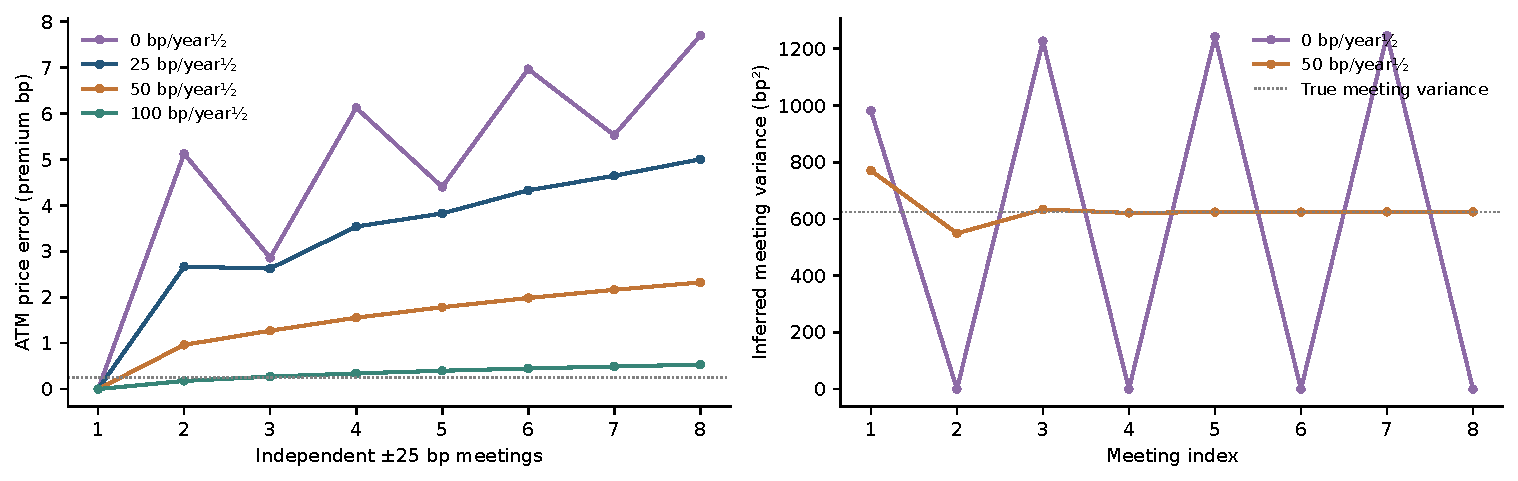
\includegraphics[width=\textwidth]{figures/atm_additivity.pdf}
\caption{Independent $\pm25$ bp meetings with Gaussian background. Left: ATM-price error from adding the identical one-increment ATM proxies; the dotted line is 0.25 bp. Right: meeting variances inferred by fitting each expiry exactly and subtracting the known background. Every actual meeting has variance 625 bp$^2$ (dotted line).}\label{fig:additivity}
\end{figure}
